\chapter{Results}\label{results}

To present our results we would like to refer to two videos created as part of the assignment. The first \ref{fig:franka-sim} was done in the Gazebo environment and it performs smoothly and in expected manner. The same could be seen in the video made in the real life setting \ref{fig:franka-real} by applying the same trajectory generators. 


\begin{figure}[htpb]
    \centering
    \includegraphics[width=0.45\textwidth]{figures/franka-sim.png}
    \caption{\href{https://gitlab.lrz.de/tum-impl-ss24/assignment2-group1/-/blob/main/media/content/gazebo-whiteboard-task-simulation.mov}{Simulation video (lrz link)}}
    \label{fig:franka-sim}
\end{figure}
\begin{figure}[htpb]
    \centering
    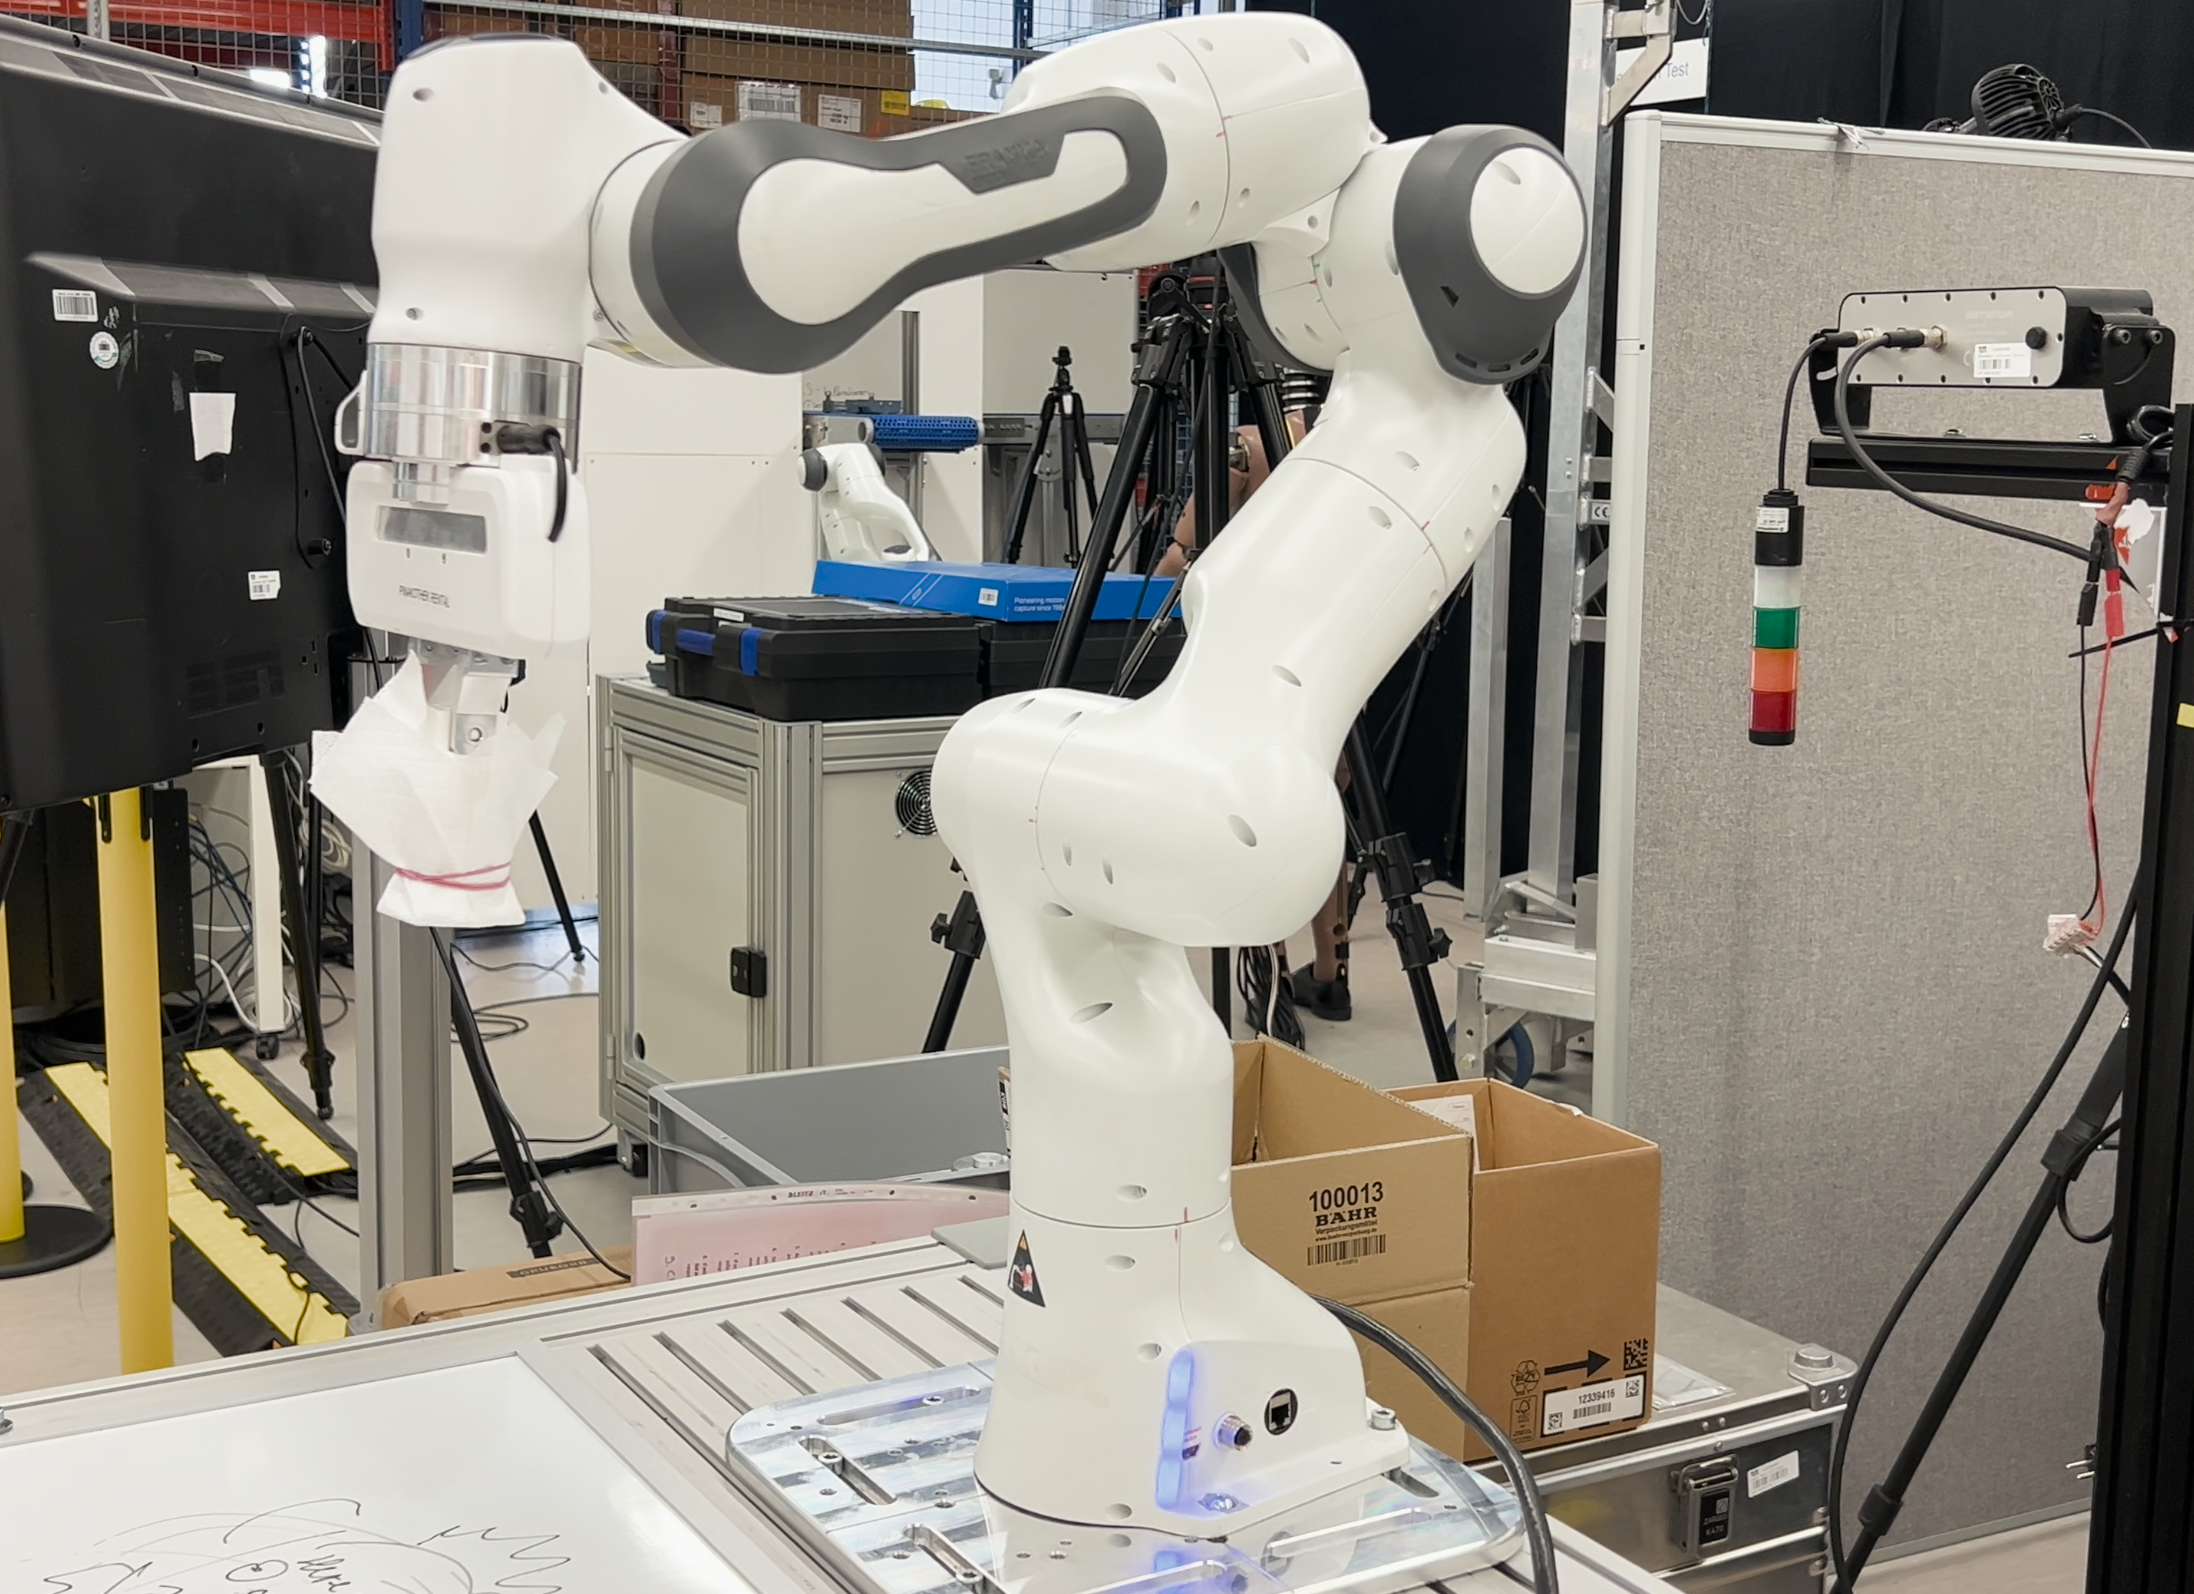
\includegraphics[width=0.45\textwidth]{figures/random-franka.png}
    \caption{\href{https://gitlab.lrz.de/tum-impl-ss24/assignment2-group1/-/raw/main/media/content/cleaning-whiteboard-task.mp4}{Linear movement towards the surface}}
    \label{fig:franka-real}
\end{figure}